\chapter{Cell Balancing}
\label{cha:balancing}
As discussed in the introduction, the problem of battery balancing can reduce net battery capacity. To realize the extent of the losses, Chimera Evoluzione's battery pack has been analyzed. Chimera Evoluzione did not feature cell balancing, but could still measure individual cell voltages and has been in use for one year without being manually balanced. \autoref{fig:chimera_imbalance} shows measured open-circuit voltages of the whole battery pack.

\begin{figure}[h]
    \centering
    \begin{tikzpicture}
    \begin{axis}[
            width=12cm,
            enlargelimits=0.02,
            xlabel=Cell number,
            ybar interval,
            ylabel=Voltage,
            xtick={0,18,36,...,108},
            bar width=4pt
        ]
        \addplot [draw=red,fill=red!60] table[x=index,y=voltage, col sep=comma]{pictures/chimera_imbalance.csv};
    \end{axis}
\end{tikzpicture}
    \caption{Unbalanced Chimera Evoluzione cells.}
    \label{fig:chimera_imbalance}
\end{figure}

As can be seen in the chart, The difference between the highest-voltage cell ($V_{max} = V_{70} = 3.712 V$) and the lowest-voltage cell ($V_{min} = V_{73} = 3.554 V$) is $V_{delta}=V_{max}-V_{min}=0.158 V$. The difference between the average voltage and the minimum and maximum voltage is respectively $V^0_{delta} = V_{avg} - V_{min} = 0.066 V$ and $V^1_{delta} = V_{max} - V_{avg} = 0.091 V$.

If the pack in those conditions is discharged until $V_{73}$ reaches the cut-off voltage of $V_{low} = 3.000 V$, the average cell voltage would be $V^0_{avg} = V_{low} + V^0_{delta} = 3.066 V $. Similarly, if the battery is charged until $V_{70}$ reaches $V_{high} = 4.200 V$, the average voltage could only reach $V^1_{avg} = V_{high} - V^1_{delta} = 4.109 V$.

Chimera Evoluzione's battery pack is a 108s6p design, with each cell rated at 9.36 Wh nominal. Considering the discharge capacity curve for a single cell at 5 A \autoref{chap:vtc5}, the capacity lost between $V_{high}$ and $V^1_{avg}$ can be approximated to 0.2 Wh, or 2.1\% of a cell's energy. The low-end capacity between $V_{low}$ and $V^0_{avg} = 3.0 V$ is close to 0.2 Wh as well. Assuming a total pack nominal energy capacity of $E_{total} = 6065.3 Wh$, the energy loss amounts to $E_{lost} = E_{total}*4.2\% = 255 Wh$. Assuming a usable capacity of $E_{total}$ during an endurance event the average energy consumption of the car should remain below $\nicefrac{E_{total}}{22 km}=275\nicefrac{Wh}{km}$ without a safety margin. If a 10\% margin is considered, the maximum consumption is $C_{max} = 248\nicefrac{Wh}{km}$. It can then be assumed that the cost of an unbalanced battery pack is $\Delta S = \nicefrac{E_{lost}}{C_{max}} = 1 km$ of range in an endurance event.

With the use of cell balancing, it is expected to get imbalance values below 10 mV between all cells, making losses irrelevant.

\section{Balancing techniques}
There are different methods to balance a battery pack; They can be summarized into passive balancing, energy transfer and individual charge control \cite{6966514}.
Passive balancing is the simplest technique to implement: it only needs a switched shunt resistor in parallel to each battery module that dissipates the excess energy from each cell. The main disadvantages are the great heat generation that requires active cooling and the reduced overall efficiency of the battery pack that loses some of its energy through the balancing process.
\begin{figure}[h]
    \centering
    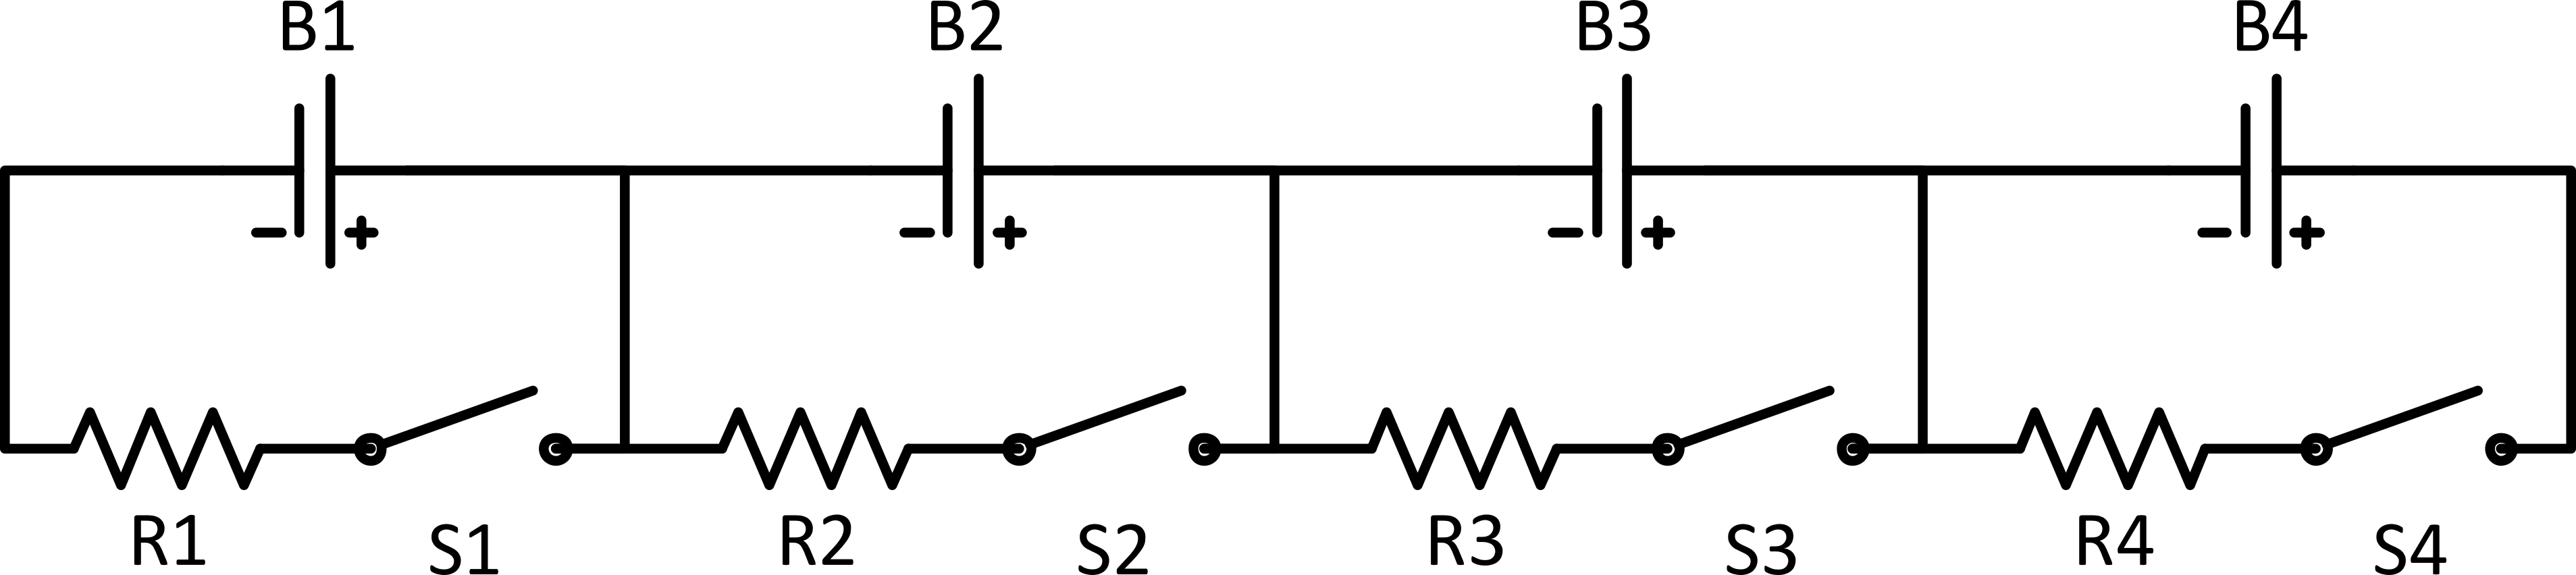
\includegraphics[scale=1.5]{passive_balancing.png}
    \caption{Passive balancing wiring schema}
    \label{fig:passive_balancing}
\end{figure}

More efficient techniques exist under the name of active balancing. As the name suggests, excess energy is not wasted using these methods.
Energy transfer is a balancing strategy that can move energy between cells of the pack. For this to work, every cell must be interconnected with each other with some circuitry. One of the simplest transfer circuits is made of capacitors that can be alternately connected in parallel to two adjacent cells. Both poles of each capacitor can be switched at the same time to be connected to either one of the two cells, charging the capacitor from one cell and discharging it on the other, using the capacitor as a bucket to transfer energy between the cells. This is the simplest active balancing method, but its simplicity has the disadvantage of being slow to transfer energy between distant cells \cite{6966514}. More capacitor tiers can be added to provide more transfer paths at the cost of scalability.

Other systems with increased complexity involve the use of transformers, buck-boost converters or more complicated methods to transfer energy between each cell with more flexibility.

In the use case of a Formula SAE car, where the battery goes through full charge and discharge cycles, the disadvantages of a passive solution are less relevant, while the increased complexity of active balancing results in more weight and failure points. If done only during charging, passive balancing doesn't affect the running efficiency of the car, as it doesn't discharge cells when the car is running. Active balancing could provide efficiency advantages if the battery doesn't get fully charged often, as happens in road cars. For these reasons, a passive balancing design was chosen.

More advanced balancing algorithms base the imbalance computation on the state of charge of the cell instead of cell voltage \cite{8834858}. This preliminary study focuses on voltage values as a reference, since the state of charge estimation is not yet implemented in the BMS.

The balancing hardware is located on the cellboards and is composed of the battery management chip that drives external transistors which can connect each battery module in parallel with a power resistor. The resulting circuit discharges the module at a rate of $400 mA$ \cite{fenice-bms-hv}.

\subsection{Strategy}
A design constraint in the balancing circuitry on the cellboards prevents two adjacent cells to be discharged simultaneously. To work around this problem an algorithm has been developed to select the optimal set of cells that can be discharged at the same time.

\begin{figure}[h]
    \centering
    \begin{tikzpicture}[->, >=stealth', shorten >= 5pt, node  distance = 2.5cm, semithick]
	\node[state, initial]	(off)                         {$Off$};
	\node[state]            (computing)      [above right=2cm of off]          {$Comp$};
	\node[state]            (discharging)  [right=1cm of off]                 {$Dsc$};
	\node[state]            (cooldown)   [below right=2cm of off]           {$Cool$};

	\path (off)      edge[bend right=10] (computing)
	edge[loop below] (off);
	\path (computing) edge (discharging)
	edge [bend right=10] (off);
	\path (discharging) edge[loop right] (discharging)
	edge (cooldown)
	edge(off);
	\path (cooldown) edge[loop left] (cooldown)
	edge[bend right=60] (computing)
	edge(off);
	%\path (pc_start)    edge (pc_wait);
	%\path (pc_wait)     edge[loop below] (pc_wait)
	%edge[bend left=5] (ts_off)
	%edge (pc_end);
	%\path (pc_end)      edge[bend left=10] (ts_on)
	%edge[bend right=10] (charge);
	%\path (ts_on)       edge[loop right] (ts_on)
	%edge[bend right=7] (ts_off);
	%\path (charge)      edge[loop left] (charge)
	%edge[bend right] (ts_off);
	%\path (stacca)      edge (halt);
	%\path (halt)        edge[loop left] (halt);
	%\path (all)         edge (stacca);
\end{tikzpicture}

    \caption{Balancing state machine}
    \label{fig:bms_fsm}
\end{figure}

When enabled, the cell balancing algorithm runs periodically following the state machine shown in \autoref{fig:bms_fsm}: first, the algorithm computes the set of cells to discharge (\textit{Comp}); The balancing ICs on the cellboards are then instructed to start the discharge process on selected cells. The discharge period lasts 30 seconds at the end of which there is a cooldown period of 10 seconds, which lets the voltages stabilize and the discharge resistors cool down. After cooldown, the algorithm is executed again. If no cells need discharging anymore, the state machine goes back to the \textit{Off} state. The balancing state machine can be stopped at all times by external events.
%Cell balancing is divided into temporal cycles of 30 seconds. At the beginning of a cycle an algorithm selects the cells to discharge and instructs the hardware which starts to discharge the cells. After the cycle's time is elapsed, the hardware stops the discharge and waits for voltages to stabilize; then the cycle repeats.\\
%A limitation in the Cellboard hardware doesn't let two adjacent cells to be discharged simultaneously. For this reason a custom algorithm has been devised to select which cells need and can be discharged.

\section{Algorithm}

The algorithm is made of two parts: the first computes the amount of imbalance of each cell compared to the minimum voltage, while the last selects the optimal combination of cells that can be discharged continuously.

\subsection{Imbalance computation}

The imbalance computation algorithm assigns an integer value $I[i]$ to each cell that equals the difference between the $i$th cell and the lowest voltage cell plus a threshold. Since passive balancing can only discharge the batteries, the minimum voltage in the pack is the target voltage.
\[
    I[i] = voltages[i] - (min(voltages) + threshold)
\]

\begin{algorithm}[H]
    \DontPrintSemicolon
    \NoCaptionOfAlgo
    \caption[imbalance]{\INTARRAY\ \textsf{imbalance}(\INTARRAY\ $voltages$, \INTEGER\ $n$, \INTEGER\ $threshold$)}\label{algorithm:imbalance}

    $I = \INTEGER[0 \ldots n-1]$\;
    $min\_voltage=\textsf{min}(voltages)$\;
    \For{$i=0 \to\ n$}{
    $I[i] = \textsf{max}(0, voltages[i] - (min\_voltage + threshold))$\;
    }
    \Return I\;
\end{algorithm}
The practical implementation cuts the imbalance to values greater than zero, as cells with negative imbalance don't need to be discharged.

\subsection{Cell Selection}
The hardware limitation discussed above poses the interesting challenge of finding the optimal combination of compatible cells that need to be discharged. The optimal combination is the one that discharges all the overcharged cells in the least amount of cycles, avoiding neighboring cells in the same discharge cycle. The problem is similar to a canonical optimization problem that can be solved efficiently with Dynamic Programming \cite{montresor}.

The problem can be formulated as follows:

Given a vector of imbalances $I[]$ of size $n$, select the smallest subset of non-adjacent cells that maximizes the sum of imbalance. The smallest subset is required to avoid cells with zero imbalance.

By using the imbalance of each cell as a priority value, the algorithm prefers highly unbalanced cells.

Let $Cells[i]$ be a subset of the first $i \le n$ indexes that respect the above requirements. Given this definition, $Cells[n]$ is the solution to the problem.

\subsubsection{Recursive step}
First, only cells with a positive imbalance ($I[i] > 0$) are considered. For these cells, two options are available:
\begin{itemize}
    \item if $i$ is selected:
          \[
              Cells[i] = \{i\} \cup Cells[i-2]
          \]
          In this case, cell $i-1$ is a neighbor of $i$ and has to be discarded, thus $i-2$ is the closest cell that can be picked.
    \item if $i$ is skipped, then $Cells[i]=Cells[i-1]$
\end{itemize}
The choice to select $i$ or not is made by comparing the resulting set for both options and picking the one with higher imbalance:
\begin{equation}
    Cells[i] = \mathit{highest}(Cells[i-1], \{i\} \cup Cells[i-2])
\end{equation}
$\mathit{highest}$ is a function that sums the imbalance of the two sets and returns the set with the highest value.

\subsubsection{Base cases}
The recursion is completed by the introduction of two base cases:
\begin{gather}
    Cells[0]=\emptyset \\
    Cells[1]=\begin{cases}
        \emptyset & I[i-1] \leq 0 \\
        \{ 0 \}   & I[i-1] > 0
    \end{cases}
\end{gather}

\subsubsection{Recursive function}
The complete solution can be expressed with the following recursive equation:
\[
    Cells[i] = \begin{cases}
        \emptyset                                           & i=0\ or\ (i=1,\ I[i-1]<0) \\
        \{i-1\}                                             & i=1, \ I[i-1] > 0         \\
        Cells[i-1]                                          & i \ge 2,\ I[i-1] \leq 0   \\
        \mathit{highest}(Cells[i-1], \{i\} \cup Cells[i-2]) & i \ge 2,\ I[i-1] > 0      \\
    \end{cases}
\]

\subsection{Implementation}

A very efficient approach to this problem is to find and save in a helper array ($C[]$) the maximum sum of imbalances for all subsets of $n$ and compatible cells, and then reconstruct the solution by walking back from it. This variation benefits from not relying on complex data structures such as sets, and it reduces computational complexity by not needing the custom $\mathit{highest}$ function for each cell that could result in an algorithm with quadratic computational complexity.

\subsubsection{Computing the maximum}
Let $C[i]$ be the maximum total imbalance from compatible cells that can be obtained with the first $i$ cells.

$C[n]$ is the solution to the problem.

\paragraph{Recursive Step}

For each cell $i$, two options can be considered:
\begin{enumerate}
    \item If cell $i$ is discarded, cell $i-1$ can be selected:
          \[
              C[i]=C[i-1]
          \]

    \item If cell $i$ is selected, cell $i-1$ has to be discarded, but $i-2$ can be selected:
          \[
              C[i]=I[i-1]+C[i-2]
          \]
\end{enumerate}

To maximize the total imbalance, the highest of the two possibilities is chosen:
\[
    C[i]=\max(C[i-1],\ I[i-1] + C[i-2])
\]

By adding the base cases, the complete recursion can be defined as follows:
\[
    C[i] = \begin{cases}
        0                                      & i=0      \\
        I[0]                                   & i=1      \\
        \mathit{\max}(C[i-1], C[i-2] + I[i-1]) & i \geq 2
    \end{cases}
\]

\subsection{Pseudo-code}
Since $\mathit{imbalance()}$ returns an array of non-negative values, there is no need to check if a certain imbalance is negative. For this reason the $\mathit{exclude()}$ function does not theck the values of $I[]$.

\begin{algorithm}[H]
    \DontPrintSemicolon
    \NoCaptionOfAlgo
    \caption[exclude]{\INTEGER\ \textsf{exclude} (\INTARRAY\ $I$, \INTEGER\ $n$)}\label{algorithm:exclude}
    $\INTARRAY\ C = \INTEGER[0 \ldots n+1]$\;

    $C[0] = 0$\;
    $C[1] = I[0]$\;

    \For{$i=2 \to\ n + 1$}{
        $C[i] = \max(C[i-1],\ C[i-2] + I[i-1])$\;
    }

    \Return $C[n]$\;
\end{algorithm}

\subsubsection{Reconstructing the set}
The \textit{exclude()} function describes a correct albeit partial solution to the problem since the set of cells to discharge is not returned. However, as discussed before, the set of selected cells can be reconstructed by analyzing the $C[]$ array in a top-down fashion.

The \textit{solution()} recursive function starts from the $C[]$ array returned by \textit{exclude()} and finds the cells that have been selected by comparing the imbalance of each cell with the relative increase in imbalance from the previous elements of the $C[]$ array.
For example, if $C[i]$ is equals to $C[i-1]$ it can be assumed that cell $i-1$ has not been selected, otherwise $C[i]$ would be greater than $C[i-1]$. In this case the output set remains unchanged and the function is called with a decremented $i$.

If the two values are different the only possibility is for cell $i-1$ to have been selected, so $\{i-1\}$ is inserted in the output set and \textit{solution()} is called again with $i$ decremented by 2. However, if $i$ equals to 1 it cannot be decremented by 2 as it will go negative. For this particular case the set $\{i-1\}$ is returned.

When $i$ reaches 0, the empty set is returned, as a starting point for the stack of pending function calls that will fill it.

\begin{algorithm}[H]
    \DontPrintSemicolon
    \NoCaptionOfAlgo
    \caption[solution]{\SET\ \textsf{solution} (\INTARRAY\ $D$, \INTEGER\ $i$)}\label{algorithm:solution}
    \uIf{i == 0}{
        \Return $\{\emptyset \}$\;
    }
    \uElseIf{$D[i] == D[i-1]$}{
        \Return $\textsf{solution}(D, i-1)$\;
    }
    \Else{
        \If{$i>1$}{
            \Return $\textsf{solution}(D, i-2) \cup \{i-1\}$\;
        }
        \Return $\{i-1\}$\;

    }
\end{algorithm}

Finally, a wrapper function \textit{balance()} calls all the above routines in the right order and with the right parameters. The variable $seg$ defines how many segments the pack is made of. In Fenice, this number corresponds to the number of cellboards.

While \textit{solution()} could simply be called once, this distinction is necessary to handle the case in which two imbalanced neighboring cells that are managed by two different cellboards need to be discharged. Although they are neighbors, these two cells are not affected by the hardware limitation of the cellboards, as they are not sharing the same balancing circuit. By calling \textit{solution()} for each subset of cells this property is respected.
\begin{algorithm}
    \DontPrintSemicolon
    \NoCaptionOfAlgo
    \caption[balancing]{\SET\ \textsf{balance} (\INTARRAY\ $voltages$, \INTEGER\ $n$, \INTEGER\ $seg$, \INTEGER\ $threshold$)}\label{algorithm:balancing}

    \INTARRAY\ $I = \textsf{imbalance}(voltages,\ threshold)$\;

    \If{$I={\emptyset}$}{
    \Return $\emptyset$\;
    }

    $\textsf{exclude}(I, n)$\;

    $sol=\emptyset$\;
    \For{$i=0 \to seg$}{
        $sol=sol \cup \textsf{solution}(I[i*(n/seg)], n/seg)$\;
    }
    \Return $sol$\;
\end{algorithm}

\subsubsection{Complexity}
It's easy to see that \textit{imbalance()}, \textit{exclude()} and \textit{solution()} are all belonging to the linear time complexity set $\Theta(n)$.
Even if \textit{solution()} is called $seg$ times, the size of data is also smaller by the same value, and with $seg$ being a constant the function still has a complexity of $\Theta(n)$.
\[
    \sum_{i=0}^{seg} \Theta(n/seg) = \Theta(n)
\]
The complete algorithm inherits the complexity from its components, thus can be categorized as $\Theta(n)$ as well.

\subsubsection{Distribution}
The modular nature of the algorithm enables the possibility of running different parts in separate systems. The mainboard is the only device that has track of all the voltages together, so it's the only one that can run \textit{imbalance()}. The list of imbalanced cells is then sent to the cellboards which execute the remaining \textit{exclude()} and \textit{solution()} functions for their subset of cells.

\newpage

